\documentclass[a4paper,14pt]{article}

\usepackage[linesnumbered, noline, noend, spanish, onelanguage, boxed]{algorithm2e}

\usepackage[colorlinks, linkcolor=blue]{hyperref}
\usepackage{indentfirst}
\usepackage[T1,T2A]{fontenc}
\usepackage[utf8]{inputenc}
\usepackage[russian]{babel}
\usepackage[fleqn]{amsmath}
\usepackage{amssymb}
\usepackage{graphicx}
\usepackage{float}
\usepackage{sectsty}

\sectionfont{\fontsize{14}{14}\selectfont}
\subsectionfont{\fontsize{14}{14}\selectfont}

\usepackage{fancyhdr}
\usepackage{titling}
\usepackage{datetime}
\usepackage{amsthm}
% \usepackage[headheight=15pt]{geometry}
\usepackage{pstricks}
\usepackage{color}
\usepackage{etoolbox}

\usepackage{caption}
%\usepackage{subcaption}

\usepackage{verbatim}
\usepackage{amsfonts}
\usepackage{epstopdf}
\usepackage[nottoc,numbib]{tocbibind}
%\usepackage[backend=bibtex,sorting=none]{biblatex}

%\addbibresourse{biblio}     %% имя библиографической базы (bib-файла) 
%\usepackage[backend=biber, style=numeric, sorting=none]{biblatex}‌​

%\geometry{left=2cm}% левое поле
%\geometry{right=1.5cm}% правое поле
%\geometry{top=1cm}% верхнее поле
%\geometry{bottom=2cm}% нижнее поле

\makeatletter
\newcommand*{\rom}[1]{\expandafter\@slowromancap\romannumeral #1@}
\DeclareMathOperator*{\argmaxA}{argmax}
%\let\oldref\ref
%\renewcommand{\ref}[1]{(\oldref{#1})}
\makeatother

%\theoremstyle{definition}
\newtheorem{defn}{Определение}
\newtheorem{theorem}{Теорема}
%\newtheorem{proof}{Доказательство}
\newtheorem{lemma}{Лемма}

\textwidth=165mm
\textheight=245mm
\oddsidemargin=5mm
\topmargin=-10mm
\parindent=0.4cm

\makeatletter
\renewcommand\@biblabel[1]{#1.}
\makeatother

\captionsetup[algorithm2e]{font=Large}

\def\labelitemi{$\triangleright$}
%\setcounter{secnumdepth}{0}

\usepackage{titlesec}
%\titleformat{\section}{\fontsize{14}{14}\selectfont\centering\bfseries}
%\titleformat{\subsection}{\fontsize{14}{14}\selectfont\centering\bfseries}

\SetKwInput{KwData}{Исходные параметры}
\SetKwInput{KwResult}{Результат}
\SetKwInput{KwIn}{Вход}
\SetKwInput{KwOut}{Выход}
\SetKwIF{If}{ElseIf}{Else}{если}{тогда}{иначе если}{иначе}{конец условия}
\SetKwFor{While}{до тех пор, пока}{выполнять}{конец цикла}
\SetKw{KwTo}{от}
\SetKw{KwRet}{вернуть}
\SetKw{Return}{вернуть}
\SetKwBlock{Begin}{начало}{конец}
\SetKwSwitch{Switch}{Case}{Other}{Проверить значение}{и выполнить}{вариант}{в противном случае}{конец варианта}{конец проверки значений}
\SetKwFor{For}{для}{:}{конец цикла}
\SetKwFor{ForEach}{для каждого}{выполнять}{конец цикла}
\SetKwFor{ForAll}{для всех}{выполнять}{конец цикла}
\SetKwRepeat{Repeat}{повторять}{до тех пор, пока}
\SetAlgorithmName{Алгоритм}{алгоритм}{Список алгоритмов}

%\usepackage{float}
%\newfloat{algorithm}{t}{lop}

\begin{document}
	%\maketitle
	%\pagestyle{fancy}
	%\fancyhead{}
	%\fancyhead[L]{\thetitle}
	%\fancyhead[R]{\thedate}
	\Large
	\IncMargin{0.8em}
	
	\begin{center}
{ \bfseries

\large{МИНОБРНАУКИ РОССИИ}

\vspace{1cm}

\large{Федеральное государственное автономное образовательное 
	учреждение}

\large{высшего образования}

\large{«Южный федеральный университет»}

\vspace{1cm}

\large{Институт математики, механики и компьютерных наук им.\\ И.И.Воровича}
 
\large{Кафедра алгебры и дискретной математики}

\vspace{2cm}

\large{Мурадьян Илья Валерьевич}

\vspace{2cm}

\LARGE{\textsc{Задача поиска графа-паттерна\\ на помеченном графе}}

\vspace{2cm}

\large{ВЫПУСКНАЯ КВАЛИФИКАЦИОННАЯ РАБОТА\\
}
\large{по направлению 01.03.02 — Прикладная математика и информатика}
\vspace{2cm}

 
\large{ 
Научный руководитель -- 

доцент,  к.ф.-м.н. Скороходов Владимир Александрович
}

\vspace{6cm}

Ростов-на-Дону -- 2018
}
\end{center}
\thispagestyle{empty}
\pagebreak
	
	\tableofcontents
	
	\newpage
	\section{Введение}
Теория графов - относительно молодой и быстроразвивающийся раздел современной математики. В ней присутствует достаточно много серьёзных теоретических проблем, таких как, например, гипотеза Харари\cite{harari} о том, что если граф имеет более трёх рёбер, то его можно однозначно восстановить по подграфам, полученным удалением единственного ребра. Но вместе с этим теория графов успешно применяется для решения прикладных задач, возникающих в теории компьютерных сетей, машинном обучении, при проектировании и эксплуатации транспортных систем, в теории игр и т.д.

Одной из классических задач теории графов является задача об изоморфизме графов. В ней даны два графа $G$ и $G'$, для которых необходимо построить два биективных отображения $\delta'$ и $\gamma$ таким образом, чтобы они переводили один граф в другой. Понятно, что такие отображения построить можно не всегда. Долгое время для этой задачи не могли найти хорошего алгоритма, и лучшей оставалась оценка $T(n) = \exp(O(\sqrt{n \log n}))$, где $n$ - число вершин, но в 2015 году Ласло Бабай опубликовал статью \cite{izom}, в которой показывается оценка $T(n) = \exp((\log n)^{O(1)})$, которая очень близка к полиномиальной. Тем не менее, приведённый в этой статье алгоритм всё ещё имеет слишком большую вычислительную сложность для того, чтобы применяться на практике для больших графов. Тем более, задача зачастую стоит немного по-другому: в графе $G$ надо найти частичный подграф \cite{berzh}, изоморфный графу $G'$, что сразу усложняет любой существующий -- переборный или более продвинутый -- алгоритм.

В приложениях, однако, часто можно ослабить условие задачи изоморфизма, определенным образом пометив вершины или дуги графов $G$ и $G'$, то есть сопоставив каждой вершине этих графов какой-то элемент множества $L$, а каждой дуге -- элемент множества $M$. В этом случае на отображения $\delta$ и $\gamma$ накладываются достаточно жесткие условия: $\delta$ может перевести $x$ в $x'$, а $\gamma$ -- $u$ в $u'$, только если вершины $x$ и $x'$ и дуги $u$ и $u'$ помечены одинаково. В случае, если множества меток $L$ и $M$ достаточно велики, количество перебираемых для отображений $\delta$ и $\gamma$ вариантов сильно сокращается, что улучшает вычислительную сложность используемых для решения этой задачи алгоритмов. 

Задачу изоморфизма помеченных графов также можно поставить более общем и полезном на практике виде: найти такой частичный подграф графа $G$, который будет изоморфен в обозначенном выше смысле графу $G'$. Такую задачу называют задачей поиска паттерна на помеченном графе.

В статье \cite{patmat} приведён алгоритм нахождения граф-паттерна на помеченном графе в случае, если дуги графа не помечены (то есть в формулировке нет множества $M$), а метки вершин графа $G'$ -- уникальны. В подготовленной мной выпускной бакалаврской работе приведено описание этого алгоритма, а также его модификация для случая, когда метки графа $G'$ не уникальны, и допускаются метки на дугах. Такая модификация расширяет применение рассмотренных в статье \cite{patmat} методов на целый класс прикладных задач. Например, при поиске паттернов на фотографиях часто бывает так, что разыскиваемый паттерн состоит из нескольких одинаковых частей. Таков, например, паттерн лица или солнцезащитных очков. Более того, на таких паттернах зачастую важно учитывать расстояние между их частями, которое отлично моделируется весами на дугах графов-паттернов. В данной работе показано, как учитывать веса на дугах графов-паттернов для нахождения соответствующего данному паттерну частичного подграфа.

Кроме распознавания образов на фотографиях, поиск паттернов на помеченных графах может использоваться и как инструмент социальной инженерии. Так, например, в 2016 году в средствах массовой информации широко освещалась деятельность так называемых групп смерти (\cite{sinkit}), получивших распространение в различных социальных сетях. При наличии полученной административными методами переписки жителей определённого города или района, можно построить граф, вершинами которого будут аккаунты пользователей, а дугами будут связаны те пользователи, которые вели друг с другом переписку. Особым образом следует пометить вершины, соответствующие аккаунтам <<целевой аудитории>> групп смерти -- подростков в возрасте от 13 до 19 лет, а также дуги, соответствующие переписке с различными стоп-словами типа <<суицид>>, <<4:20>> и пр. После этого следует составить граф-паттерн, выглядящий, например, как граф-звезда (т.е. связный граф, степень всех вершин которого, кроме одной, равна 1 \cite{stargraph}) с 10 листьями-подростками, а дуги графа-паттерна должны быть помечены в обозначенном выше смысле. После того, как паттерн построен, можно применить алгоритм из данной работы и найти все соответствующие ему подграфы, после чего, проводя их анализ, установить координаторов <<групп смерти>>.

Все представленные в данной работе алгоритмы были реализованы на языке Python с использованием библиотеки GraphTool. Оба этих проекта -- проекты с открытым исходным кодом и исключительно полной документацией (\cite{pythdoc}, \cite{graphtool}), которая достаточно активно использовалась в процессе разработки. Для контроля версий и работы за разными машинами также использовалась система контроля версий Git, исходный код которой также открыт. Несмотря на обилие открытых источников, для более подробного ознакомления с этой системой я выбрал книгу \cite{gitbook}.
	
	%\newpage
	\section{Основные понятия}
Ниже приведены основные понятия и утверждения, необходимые для дальнейшего изложения \cite{berzh}.

\begin{defn}
	Ориентированным графом будем называть двойку\\ $G (V, E)$, где:
	\begin{itemize}
		\item $V, |V|>0$ - множество вершин графа;
		\item $E \subset V \times V$ - множество дуг графа;
	\end{itemize}
\end{defn}
\begin{defn}
	Неориентированным графом будем называть двойку\\ $G (V, E)$, где:
	\begin{itemize}
		\item $V, |V|>0$ - множество вершин графа;
		\item $E \subset V \times V$ - множество дуг графа;
		\item $\forall u, v \in V: \quad (u, v) \in E \Leftrightarrow (v, u) \in E$
	\end{itemize}
\end{defn}

Нам также потребуется определение обратных дуг.

\begin{defn}
	Если $e_1 = (u, v) \in E, e_2 = (v, u) \in E$, то дуги $e_1$ и $e_2$ называют обратными.
\end{defn}

Из определений следует, что неориентированный граф с хотя бы одной дугой содержит по крайней мере одну пару обратных дуг.

Все определения в данном разделе применимы как для ориентированных, так и для неориентированных графов.

\begin{defn}
	Граф $G(V, E)$ будем называть конечным, если множества $V$ и $E$ конечны.
\end{defn}
\begin{defn}
	Тройку $G(V, E, \omega)$ будем называть взвешенным графом, если $G'(V, E)$ -- граф, а $\omega : E \to \mathbb{R}$ -- весовая функция.
\end{defn}
\begin{defn}
	Будем говорить, что дуга $e = (u, v)$ исходит из вершины $u$ и заходит в вершину $v$. Вершину $u$ будем называть началом, а $v$ -- концом дуги.
\end{defn} 
\begin{defn}
	Будем говорить, что вершина $u$ смежна с вершиной $v$, если существует дуга $e = (u,v) \in E$. Обозначим множество вершин, смежных с $u$, через $\Gamma(u)$. Обозначим также $\Gamma^{-1}(u) = \{v | \exists (v, u) \in E \} $. Множество $Inc(u) = \{(u, v) \in E | v \in V \}$ назовём множеством инцидентных $u$ дуг.
\end{defn} 

Заметим, что для неориентированных графов для любой вершины $u$ выполнено $\Gamma(u) = \Gamma^{-1}(u)$.

Введём понятия пути и цепи.

\begin{defn}
	Путём называется последовательность дуг $\mu = (e_i = (u_i, u_{i+1}))_{i = 0}^{m-1}$. Число $m$ назовём длиной пути и обозначим через $|\mu|$. Будем говорить, что $\mu.s = u_0$ -- это начало пути $\mu$, а $\mu.t = u_m$ -- это конец пути $\mu$. Путь ненулевой длины $\mu$ называется контуром, если его начало совпадает с концом. Простым называется контур, не содержащий одинаковых или обратных дуг. Если граф не содержит простых контуров, он называется бесконтурным.
\end{defn} 

Также приведём определение цепи.

\begin{defn}
	Цепью на графе $G$ называется последовательность дуг $\lambda = (e_i)_{i = 0}^{m-1}$ такая, что для любого $i \in [0;m-2]_\mathbb{N}$ дуги $e_i$ и $e_{i+1}$ имеют ровно одну общую вершину (но необязательно начало дуги $e_i$ совпадает с концом $e_{i+1}$). Число $m$ назовём длиной цепи и обозначим через $|\lambda|$. Будем говорить, что вершина дуги $e_0$, не инцидентная дуге $e_q$ -- это начало цепи $\lambda$, а вершина дуги $e_{m-1}$, не инцидентная дуге $e_{m-2}$ -- это конец цепи $\lambda$. Цепь ненулевой длины $\lambda$ называется циклом, если её начало совпадает с концом.
\end{defn} 

Необходимо также ввести некоторые определения, специфичные для данной работы.

\begin{defn}
	Расстоянием $d(u, v)$ между вершинами графа $u$ и $v$ называется длина наименьшего пути, началом которого является вершина $u$, а концом - вершина $v$, или наоборот. Если ни одного такого пути не существует, то расстояние между вершинами полагается равным бесконечности.
\end{defn}

\begin{defn}
	Неориентированным расстоянием $dn(u, v)$ между вершинами графа $u$ и $v$ называется длина наименьшей цепи, началом которой является вершина $u$, а концом - вершина $v$. Если ни одной такой цепи не существует, то неориентированное расстояние между вершинами полагается равным бесконечности.
\end{defn}

\begin{defn}
	Диаметром $diam(G)$ связного графа $G$ называется максимальное из неориентированных расстояний между его вершинами.
\end{defn}

Заметим, что в связном конечном графе неориентированные расстояния между любыми двумя вершинами всегда конечны, поэтому и диаметр такого графа также будет конечен. В данной работе мы будем рассматривать лишь связные и конечные графы, поэтому все они будут иметь конечный диаметр.

Нам также понадобятся определения, связанные с подграфами и частичными графами.

\begin{defn}
	 Граф $G'(V', E')$ называется частичным графом графа $G(V, E)$, если $V' = V, E' \subset E$.
\end{defn}

\begin{defn}
	Граф $G'(V', E')$ называется подграфом графа $G(V, E)$, если $V' \subset V, E' = \{(v, u) \in E | v \in V', u \in V'\}$.
\end{defn}

\begin{defn}
	Граф $G'(V', E')$ называется частичным подграфом графа $G(V, E)$, если $G'$ является частичным графом некоторого подграфа графа $G$.
\end{defn}
	%\input{erdesh}
	%\newpage
	\section{Задача о поиске паттерна на помеченном графе}

\subsection{Постановка задачи}
\par Пусть $L$ -- непустое конечное множество \textbf{(множество меток)}. Пусть $G(V, E)$, $G'(V', E')$ -- ориентированные связные графы. Для удобства дальнейшего изложения граф $G$ будем называть архивным графом, а граф $G'$ -- графом-паттерном, или шаблонным графом.

Введём отображения $l : V \to L$, $l' : V' \to L$, сопоставляющие вершинам архивного и шаблонного графов соответствующие метки. При этом мы требуем, чтобы введённые на шаблонном графе метки были уникальны, т.е. отображение $l'$ -- инъективно. 

Для формулировки задачи нам потребуется определение совпадения.

\begin{defn}
	Совпадением на графе $G$ будем называть частичный подграф $\widehat{G}(\widehat{V}, \widehat{E})$ графа $G$ такой, что:
	\begin{enumerate}
		\item Существует биективное отображение $m_{\widehat{G}}: V' \to \widehat{V}$.
		\item $\forall v' \in V': l'(v') = l(m_{\widehat{G}}(v'))$
		\item $\forall (v^{\prime}_1, v^{\prime}_2) \in E': (m_{\widehat{G}}(v^{\prime}_1), m_{\widehat{G}}(v^{\prime}_2)) \in E$
	\end{enumerate}
\end{defn} 

Пусть существует некоторое совпадение  $\widehat{G}(\widehat{V}, \widehat{E})$ на графе $G$ такое, что есть вершина $v \in V : v \in \widehat{V}$. Тогда вершину $v$ будем называть подходящей паттерну $G'$ по совпадению $\widehat{G}$, или истинным кандидатом, иначе -- неподходящей. В случае, если вершина $v$ подходит паттерну $G'$ по совпадению $\widehat{G}$, вершину $m_{\widehat{G}}^{-1}(v) \in  V'$ назовём соответствующей данной вершине $v$. Заметим, что вершина $v$ может подходить паттерну по нескольким совпадениям, но в силу инъективности отображения $l'$ ей может соответствовать лишь одна вершина $v' \in  V'$.

Рассмотрим задачу нахождения множества $\widetilde{V} \subseteq V$ всех подходящих паттерну $G'$ вершин.

\subsection{Алгоритм исключения по локальным условиям}

Для решения поставленной задачи будем использовать следующий алгоритм.

Пусть $T = \{\emptyset\} \cup \mathcal{C}_{V'}^1$ -- все 0-элементные и 1-элементные подмножества множества вершин графа-паттерна. Построим отображение $f_0 : V \to T$, заданное следующим:
\begin{equation}
f_0(v) = \{v' \in V' | l(v) = l'(v')\} .
\end{equation}

Нетрудно убедиться, что в силу инъективности отображения $l$, введённое отображение $f_0$ действительно имеет областью значений множество $T$.

Алгоритм исключения по локальным условиям будет строиться на изменении отображения $f_0$, поэтому для удобства нам потребуется ввести операцию над подобными отображениями. Пусть $f_1, f_2 : V \to 2^{V'}$. Обозначим $f_2 = Exclude(f_1,\allowbreak v_0 (\in V), \allowbreak v^{\prime}_0 (\in V'))$, если выполнено следующее:
\begin{enumerate}
	\item $\forall v \ne v_0 \in V: f_1(v) = f_2(v)$.
	\item $v^{\prime}_0 \notin f_2(v_0)$.
	\item $\{v^{\prime}_0\} \cup f_2(v_0) = f_1(v_0)$
\end{enumerate}

Ясно, что по отображению $f_1$ легко построить отображение $Exclude(f_1,\allowbreak v_0,\allowbreak v^{\prime}_0)$, просто исключая вершину $v^{\prime}_0$ из множества $f_1(v_0)$.

Прежде чем привести алгоритм, введём ещё несколько определений.

\begin{defn}
	Пусть дан граф $G(V, E)$. Если $\widetilde{V} \subset V$, то $\Gamma(\widetilde{V}) = \bigcup\limits_{\widetilde{v} \in \widetilde{V}} \Gamma(\widetilde{v})$. В частности, $\Gamma(\emptyset) = \emptyset$.
\end{defn} 

\begin{defn}
	Пусть $G(V, E)$, $G'(V', E')$ -- архивный и шаблонный графы соответственно. Пусть задано отображение $f : V \to T$, где множество $T$ определено выше. Путь также $v \in V$. Назовём предикатом локальных условий следующий предикат:
	\begin{equation}
		LCC(f, v) = \forall u' \in \Gamma(f(v)) \exists u \in \Gamma(v) : u' \in f(u).
	\end{equation} 
\end{defn} 

Алгоритм исключения по локальным условиям принимает на вход отображение $f_0$, сопоставляющее вершинам графа их вершины-кандидаты в графе-паттерне. На каждой итерации цикла для каждой вершины $v \in V$ выполнено $f_{i}(v) \subset f_{i-1}$. На каждой итерации $i$ из списка кандидатов исключаются те вершины $v$, для которых оказывается, что хотя бы для одной из вершин $u' \in \Gamma(f_i(v))$ не существует такой вершины $u \in \Gamma(v)$, что $f(u) = u'$. Схожая идея используется в различных классических алгоритмах теории графов, например, в алгоритме Беллмана-Форда \cite{bellmanford}. Следуя той же схеме доказательства, которая используется, например, при обосновании того факта, что алгоритм Беллмана-Форда находит на бесконтурном графе кратчайшие пути за количество итераций, равное диаметру графа, мы придём к тому, что для бесконтурного графа $G'$ алгоритм $LCCE$ отработает за $diam(G')$ итераций, после чего все вершины $v \in V$, для которых $f(v)$ не пусто, будут действительно вершинами некого графа-совпадения, ведь для каждой вершины $u = f(v)$, каждый начинающийся в ней путь (а в силу бесконтурности графа, этот путь конечный, и его длина не превышает диаметра графа) имеет некий соотносящийся с этим путём путь в графе $G$, начинающийся в вершине $v$. Для бесконтурного графа можно отдельно не вычислять его диаметр, просто прервав алгоритм после итерации $i$, для которой $F_i = F_{i-1}$.

Псевдокод алгоритма исключения по локальным условиям приведён ниже (алгоритм \ref{alg:LCCE}).

\begin{algorithm}[H]
	\Large
	\KwIn{графы $G(V, E)$, $G'(V', E')$, отображение $f_0 : V \to T$, число итераций $N$}
	\KwOut{измененённое отображение $f_K$}
	\Begin(LCCE){
		$K := 0$
		
		$F_0 := f_0$
		
		\For{$i = 1, 2, .., N$}{
			\For{$v \in V$}
			{
				\If{$\neg LCC(f_i, v)$}
				{	
					$S := K$
					
					\For{$v' \in f_S(v)$}{
						$f_{K+1} := Exclude(f_{K}, v, v')$
						
						$K := K + 1$
					}
				}
			}
		
			$F_i := f_K$
		}
		\Return{$f_N$}
	}

	\caption{Алгоритм исключения по локальным условиям}
	\label{alg:LCCE}
\end{algorithm}

Для графов-паттернов с контурами применение только этого алгоритма не даёт требуемого результата. На таких графах существуют бесконечные пути, а потому для них применение приведённого выше алгоритма со сколь угодно большим числом итераций не гарантирует того, что оставшиеся вершины-кандидаты будут в действительности вершинами некоторого графа-совпадения. Поэтому для графов с контурами мы будем применять, помимо алгоритма $LCCE$, ещё и алгоритм проверки контуров, описанный ниже.

\subsection{Алгоритм проверки контуров}

Пусть $\mathcal{K}_0$ -- это набор контуров графа $G'$. В этот набор достаточно включить все простые контуры этого графа. 
Пусть $\mathcal{C}_0 \in \mathcal{K}_0$ -- какой-то из рассматриваемых контуров. Тогда если $\mathcal{C}_0 = ((v_0', v_1'), ..., (v_{r-1}^{\prime}, v_0^{\prime}))$ и $v_0^{\prime} \in f(v_0)$, то алгоритм проверки контуров \ref{alg:CCE}, приведённый ниже, исключит вершину $v_0^{\prime}$ из множества $f(v_0)$, если окажется, что нет контура, начинающегося в вершине $v_0$ и соответствующего (в смысле отображения $f$) контуру $\mathcal{C}_0$.

\begin{algorithm}[H]
	\Large
	\KwIn{графы $G(V, E)$, $G'(V', E')$, отображение $f_0 : V \to T$}
	\KwOut{измененённое отображение $f_N$}
	\Begin(CCE){
		$K := 0$
		
		\ForEach{$\mathcal{C}_0 \in \mathcal{K}_0$}{
				Пусть $(v_0^{\prime}, v_1^{\prime})$ -- первая дуга контура $\mathcal{C}_0$.
			
			 	$\mathcal{A} := \emptyset$
			 	
			 	$\mathcal{A}_0 := \emptyset$
			 
			 	\ForAll{$v_0: f_K(v_0) \ne \emptyset$}{
			 		$\mathcal{A}_0 := \mathcal{A}_0 \cup \{v_0\}$
			 		
			 		$\mathcal{A} := \mathcal{A} \cup \{(v_0, v_0, 0)\}$
		 		}
	 		
	 			\For{$s = 1, 2, ..., |\mathcal{C}_0|$}{
		 			Пусть $(q_0, q_1)$ -- $s$-я дуга контура $\mathcal{C}_0$.
		 			
	 				$\mathcal{B} := \emptyset$
	 				
	 				\ForEach{$(v, v_0, s - 1) \in \mathcal{A}$}{
	 					\For{$v^{\prime} \in \Gamma(v) $}{
	 						\If{$q_1 \in f_K(v^{\prime})$}{
	 							$\mathcal{B} := \mathcal{B} \cup \{(v^{\prime}, v_0, s)\}$
 							}
 						}
 					}
 				
	 				$\mathcal{A} := \mathcal{B}$
	 			}
	 			
	 			
	 			\ForEach{$v_0 \in \mathcal{A}_0$}{
	 				\If{$ (v_0, v_0, |\mathcal{C}_0|) \notin \mathcal{A} $}{
	 					$S := K$
	 					
	 					\For{$v' \in f_S(v_0)$}{
	 						$f_{K+1} := Exclude(f_{K}, v_0, v')$
	 						
	 						$K := K + 1$
	 					}
 					}
	 			}
		}
		\Return{$f_N$}
	}

	\caption{Алгоритм проверки контуров}
	\label{alg:CCE}
\end{algorithm}

Нахождение всех контуров графа и такой их обход -- задачи с очень высокой вычислительной сложностью, но на практически встречающихся графах, тем не менее, основная работа будет сделана алгоритмом $LCCE$. Впрочем, можно даже рассматривать не все циклы -- можно попытаться выделить подграф совпадения и по неточному списку кандидатов. Здесь много зависит от конкретного вида графов и стоящей перед нами задачи.

Авторы статьи \cite{patmat} ожидают, что граф-паттерн будет содержать достаточно мало циклов, поэтому приводимая ими оценка сложности $O(|\mathcal{K}_0|\allowbreak n_t \allowbreak (|V| + |E|))$ является удовлетворительной. Здесь $n_t$ определяется следующим образом. Если $n_{\mathcal{C}_0}$ -- это количество вершин в $V$, соответствующих контуру $\mathcal{C}_0$, то $n_t = \max\limits_{\mathcal{C}_0 \in \mathcal{K}_0} n_{\mathcal{C}_0}$. Т

\subsection{Общий алгоритм исключения вершин-кандидатов}

Два вышеприведённых алгоритма объединяются в алгоритме \ref{alg:EE}, который выполняется до тех пор, пока из отображения $f$ ещё удаляются какие-то вершины-кандидаты.

\begin{algorithm}
	\Large
	\KwIn{графы $G(V, E)$, $G'(V', E')$, отображение $f_0 : V \to T$}
	\KwOut{измененённое отображение $f_N$}
	\Begin(Exclusion){
		$K := 0$
		
		\While{$K = 0$ или $f_K \ne f_{K - 2}$}{
			$f_{K+1} := LCCE(G, G', f_{K})$
			
			$f_{K+2} := CCE(G, G', f_{K+1})$
			
			$K := K + 2$
		}
		\Return{$f_K$}
	}

	\caption{Алгоритм исключения вершин-кандидатов}
	\label{alg:EE}
\end{algorithm}

Формируя начальное отображение $f_0$ исходя из совпадений по меткам архивного графа и графа-паттерна, мы передаём его алгоритму Exclusion и получаем на выходе новое отображение $f_N$ такое, что для любой вершины $v \in V$ каждая вершина множества $f_N(v)$ имеет вершину $v$ истинным кандидатом.

	%\section*{Частные случаи}
\par Пусть $S =\{b \in \mathbb{B}\ |\ q(b)\ne 0\}$ - множество допустимых конфигураций. Пусть также $\mathfrak{X} = M_{|S|}([0;1])$ - множество квадратных матриц порядка $|S|$ с элементами из $[0;1]$. Элементы матрицы $\chi \in \mathfrak{X}$ будем обозначать так: $\chi_{b_s,b_f}$, где $b_s, b_f \in S$. Теперь придадим этим матрицам некоторый смысл в рамках нашей задачи. 
\par Каждой паре вершин $s, f \in X$ поставим в соответствие матрицу $\chi(s,f) \in \mathfrak{X}$ такую, что число $\chi_{b_s,b_f}$ означает вероятность того, что начав движение из вершины $s$ в конфигурации $b_s$ можно добраться в вершину $f$ в конфигурации $b_f$. 
\par Легко видеть, что задача в первоначальной постановке сводится к задаче определения матрицы $\chi$ для пары из начальной и конечной вершин, и последующему вычислению суммы $\sigma = \sum\limits_{b\in S} \chi_{b_s,b}$, где $b_s$ - стартовая конфигурация. $\sigma$ и будет ответом на задачу.
\par Найдём теперь такую матрицу для некоторых пар вершин на некоторых специальных графах. Для простоты рассмотрим лишь частный случай общей задачи. Пусть $G(X, U, f)$ - граф с условиями как указано выше, причём $U = U_0 \cup U_R \cup U_G$,\\ $S = \left\{\begin{pmatrix}
0\\ 
1
\end{pmatrix},
\begin{pmatrix}
1\\ 
0
\end{pmatrix}
 \right\}$. 
	%\section*{Определение вероятности достижимости}
\begin{algorithm}
	\KwIn{$G(V,U); a, b \in V; p, q, bs \in \mathbb{B}$}
	\Begin{
		$\forall v \in V\setminus \{b\}, \forall c \in [1,n]_\mathbb{N}: prob[v][c] := 0$\\
		$\forall  c \in [1,n]_\mathbb{N}: prob[b][c] := 1$\\
		\While{$prob[a][bs]$ недостаточно точна}
		{
			\ForEach{$u = (v_0,v_1) \in U (u \in U_{col})$}
			{
				\ForEach{ $bc \in \mathbb{B} $}{
					\If{$col = 0$ OR $bc_{col} = 1$}{
						$prob[v_0][bc] = max (prob[v_0][bc], (1-p)\cdot prob[v_1][bc] + \sum\limits_{b \ne bc} \frac{prob[v_1][b]\cdot q(b)}{1-q(bc)})$
					}
				}
			}	
		}
		
	}
\end{algorithm}
	%\section*{Топологическая сортировка ациклического графа}
\par Ниже приведён нерекурсивный вариант алгоритма топологичечкой сортировки ациклического графа, который потребуется нам в алгоритме нахождения вероятности достижимости между двумя вершинам в ациклическом графе. Здесь под $G[i][c]$ подразумевается список вершин, связанных с вершиной $i$ дугами, допускающими цвет $c$. Например, чёрные дуги допускают все цвета, поэтому соответствующие вершины будут представлены в каждом из списков.


	%\newpage
	\section{Модифицированная задача}

\subsection{Постановка задачи}
\par Пусть, как и прежде, $L$ -- непустое конечное множество, называемое \textbf{множеством меток}. Пусть $G(V, E)$, $G'(V', E')$ -- ориентированные графы. Граф $G'$, кроме того, связный. Будем называть граф $G$ архивным графом, граф $G'$ -- графом-паттерном, или шаблонным графом.

Введём отображения $l : V \to L$, $l' : V' \to L$, сопоставляющие вершинам архивного и шаблонного графов соответствующие метки. Никаких дополнительных требований на эти отображения мы уже не накладываем.

Пусть также $\mathcal{X}$ -- это непустое (возможно, бесконечное) множество \textbf{(множество характеристик)} с заданным на нём бинарным отношением $\rho:\mathcal{X} \times \mathcal{X} \to \{0, 1\}$

Мы вводим множество характеристик для того, чтобы, например, работать со взвешенными графами. Действительно, если положить 

\[\mathcal{X} = \mathbb{R}\], 
\[\rho(x, y) = \begin{cases}
1, & |x - y| < \varepsilon \\
0, & |x - y| \ge \varepsilon
\end{cases}, \varepsilon > 0\],

мы получим отношение $\rho$, заданное, как отношение <<примерного равенства>>. Его мы и будем использовать для сравнения весов дуг архивного графа и графа-паттерна.

Введём также <<помечающие отображения>> для дуг графа: $\chi : E \to \mathcal{X}$, $\chi' : E' \to \mathcal{X}$.

Несколько изменится и определение совпадения.

\begin{defn}
	Совпадением на графе $G$ будем называть частичный подграф $\widehat{G}(\widehat{V}, \widehat{E})$ графа $G$ такой, что:
	\begin{enumerate}
		\item Существует биективное отображение $m_{\widehat{G}}: V' \to \widehat{V}$.
		\item $\forall v' \in V': l'(v') = l(m_{\widehat{G}}(v'))$
		\item $\forall e' = (v^{\prime}_1, v^{\prime}_2) \in E': \rho(\chi'(e'), \chi((m_{\widehat{G}}(v^{\prime}_1), m_{\widehat{G}}(v^{\prime}_2)))) = 1$
		\item $\forall (v^{\prime}_1, v^{\prime}_2) \in E': (m_{\widehat{G}}(v^{\prime}_1), m_{\widehat{G}}(v^{\prime}_2)) \in E$
	\end{enumerate}
\end{defn} 

Пусть для вершины $v \in V$ существует некоторое совпадение  $\widehat{G}(\widehat{V}, \widehat{E})$ на графе $G$ такое, что $v \in \widehat{V}$. Тогда вершину $v$ будем называть подходящей паттерну $G'$ по совпадению $\widehat{G}$, иначе -- неподходящей. В случае, если вершина $v$ подходит по совпадению $\widehat{G}$, вершину $m_{\widehat{G}}^{-1}(v) \in  V'$ назовём соответствующей данной вершине $v$.

Через $\widetilde{V} \subseteq V$ обозначим множество всех подходящих паттерну $G'$ вершин. Наша задача и будет состоять в отыскании этого подмножества. Опишем используемый нами алгоритм.

Пусть $T = \emptyset \cup \mathcal{C}_{V'}^1$ -- все подмножества множества вершин графа-паттерна. Построим отображение $f_0 : V \to T$, заданное следующим:
\begin{equation}
v' \in f_0(v) \Leftrightarrow l(v) = l'(v').
\end{equation}

Нетрудно убедиться, что в силу инъективности отображения $l$, введённое отображение $f_0$ действительно имеет областью значений множество $T$.

Алгоритм будет строиться на изменении отображения $f_0$, поэтому для удобства нам потребуется ввести операцию над подобными отображениями. Пусть $f_1, f_2 : V \to 2^{V'}$. Обозначим $f_2 = Exclude(f_1, v_0 (\in V), v^{\prime}_0 (\in V'))$, если выполнено следующее:
\begin{enumerate}
	\item $\forall v \ne v_0 \in V: f_1(v) = f_2(v)$.
	\item $v^{\prime}_0 \notin f_2(v_0)$.
	\item $\{v^{\prime}_0\} \cup f_2(v_0) = f_1(v_0)$
\end{enumerate}

Ясно, что по отображению $f_1$ легко построить отображение $Exclude(f_1, v_0, v^{\prime}_0)$, просто исключая вершину $v^{\prime}_0$ из множества $f_1(v_0)$.
\subsection{Измененный алгоритм исключения по локальным условиям}

\subsection{Измененный алгоритм проверки циклов}
	%\subsection{Решение задачи для бесконтурного случая}
\par Мы ограничимся решением задачи в случае, когда цветной граф G не содержит контуров. Введём на множестве $X$ вершин этого графа отношение $\preceq$: $x \preceq y$ тогда и только тогда, когда существует путь из вершины $x$ в вершину $y$, либо $x = y$. Известно, что введённое отношение на множестве вершин бесконтурного графа является отношением частичного порядка. Какое-либо упорядочение вершин $(x_1, x_2, ..., x_{|X|})$, для которого $\forall i, j \quad i < j \Rightarrow \neg (x_j \preceq x_i)$, назовём \textbf{топологической сортировкой} графа $G$. Известно, что для бесконтурного графа существует по крайней мере одна топологическая сортировка его вершин. Далее будем предполагать, что $(x_1, x_2, ..., x_{|X|})$ -- некоторая топологическая сортировка вершин графа $G$.
\par Напомним, что $t$ и $s$ -- начальная и конечная вершины рассматриваемого нами пути. Найдём $a, b \in \{1, 2, ..., |X|\}$ такие, что $x_a = s, x_b = t$. Если $a > b$, задача не имеет решения, поскольку не существует пути из $x_a$ в $x_b$ даже в обычном смысле. Далее будем считать, что $a \leq b$.
\par Введём в рассмотрение для каждой вершины $x_n, a \leq n \leq b$ матрицу вероятностей $P^{(n)} \in \mathbb{M}_{M \times M}$ такую, что $P^{(n)}_{i,j}$ - это вероятность оказаться в вершине $t$ в цвете $j$, начав движение из вершины $x_{n}$ в цвете $i$, и выбрав оптимальную стратегию движения. Непосредственно из определения следует, что $P^{(n)} = E$, где $E$ - единичная матрица.
\par Для нахождения остальных матриц $P^{(n)}$ мы будем использовать метод полной индукции, переходя от $(n + 1), (n + 2), ..., b$ к $n$. Пусть путешественник находится в вершине $x_n$ в цвете $i$. Тогда он может перейти по любой из дуг, допускающих этот цвет, то есть по любой из дуг множества $Inc_i(x_n)$. Пусть $\hat{X_i}(x_n)$ -- множество концов этих дуг. Путешественник не должен рассматривать в качестве кандидатов на переход те вершины $x_k \in \hat{X_i}(x_n)$, для которых $k > b$, поскольку после такого перехода вероятность оказаться в вершине $t = x_b$ окажется равной нулю. Заметим, что обязательно $k > n$, поскольку вершины графа топологически упорядочены. Поэтому множество вершин-кандидатов можно описать следующим образом: $X_i(x_n) = \{x_k \in \hat{X_i}(x_n) | n < k \leq b\}$. Если это множество пусто, то вероятность попасть в вершину $t$, находясь в цвете $i$, равна нулю, т.е. $\forall j \: P^{(n)}_{i,j} = 0$. Далее будем считать, что $X_i(x_n) \ne \emptyset$.
\par Пусть путешественник выбрал для перехода вершину $x_k \in X_i(x_n)$. Тогда матрица вероятностей для вершины $x_n$ при условии перехода в вершину $x_k$ будет равна $P^{(x_n, x_k)} = P \cdot P^{(k)}$. Это следует непосредственно из формулы полной вероятности.
\par Теперь необходимо выяснить, какую именно из вершин множества $X_i(x_n)$ должен выбрать путешественник. Мы договорились, что нашей целью является максимизация вероятности достигнуть конечной вершины $t$, при этом не имеет значения цвет, в котором эта вершина будет достигнута. Поэтому вершину для перехода необходимо выбирать так: 
\[v_i = \argmaxA_{x_k \in X_i(x_n)} \sum_{l = 1}^{M} P^{(x_n, x_k)}_{il}.\]
Таким образом, стратегия при нахождении в $i$-м цвете в вершине $x_n$ будет заключаться в выборе для перехода вершины $v_i$, а $i$-я строка искомой матрицы $P^{(n)}$ будет равна $i$-й строке матрицы $P^{(x_n, v_i)}$. Более формально, 

\[\forall j \: P^{(n)}_{i, j} = P^{(x_n, v_i)}_{i, j}, v_i = \argmaxA_{x_k \in X_i(x_n)} \sum_{l = 1}^{M} P^{(x_n, x_k)}_{il}.\]

\par Для решения задачи предлагается использовать следующий алгоритм:
\begin{enumerate}
	\item $\forall n > b: P^{(n)} := 0$.
	\item $P^{(b)} := E$.
	\item Для $n = b - 1, b - 2, ..., a$:
	\begin{enumerate}
		\item Инициализируем $P^{(n)} := 0$.
		\item Для всех $i = 1..M$:
		\begin{enumerate}
			\item Определим множество концов дуг, допускающих цвет $i$ -- $X_i(x_n)$.
			\item Если $X_i(x_n) \ne \emptyset$:
			\begin{enumerate}
				\item Для каждой вершины множества $x_k \in X_i(x_n)$ вычислим \mbox{$i$-ю} строку матрицы $P^{(x_n, x_k)}$ как указано выше, а также вероятность достижимости как сумму элементов этой строки: 
				\[p^{(x_n, x_k, i)} = \sum_{l = 1}^{M} P^{(x_n, x_k)}_{il}.\]
				\item Найдём вершину $v_{i, n} = \argmaxA_{x_k \in X_i(x_n)} p^{(x_n, x_k, i)}$.
				\item Присвоим: $\forall j = 1..M \! \!: P^{(n)}_{i, j} = P^{(x_n, v_{i, n})}_{i, j}$
			\end{enumerate}
			\item Если $X_i(x_n) = \emptyset$, установим $v_{i, n} = \bigotimes$. Это будет означать, что находясь в цвете $i$, из вершины $x_n$ добраться до конечной вершины невозможно. 
		\end{enumerate}
	\end{enumerate} 
	\item Возвращаем $P^{(a)}$ как искомую матрицу вероятностей для вершины $s$, а также набор вершин $(v_{i, n})_{a \le n < b, i \in C}$ как искомую стратегию.
\end{enumerate}

\par Очевидно, что алгоритм всегда заканчивается. Корректность алгоритма вытекает из описания, приведённого выше.
\par Определим теперь временную сложность алгоритма.
\par Первый и второй шаги алгоритма отрабатывают за время $O(M^2)$. На третьем шаге наиболее трудным является вычисление строк матрицы вероятностей. Вычисление одной такой строки занимает время $O(M^2)$. Количество таких вычислений: 

\[ S = \sum\limits_{n = a}^{b} \sum\limits_{i = 1}^{M} |X_i(x_n)| \le (b - a + 1) \cdot M \cdot \max\limits_{n, i} |X_i(x_n)|\]. 

Поскольку $(b - a + 1) \le |X|$, $\max\limits_{n, i} |X_i(x_n)| \le |X|$, то $S \le M |X|^2$. Поэтому общая сложность алгоритма составит $O(M^3 |X|^2)$.

\begin{comment}
\begin{lemma}
	В строках 3-9 функции $GetProbabilities$ вычисляются корректные вероятности достижимости для всех вершин, следующих за t в порядке топологической сортировки и для самой вершины t.
\end{lemma}
\begin{proof}
	Действительно, в строках 3-7, всем вершинам, начиная с последней вершины в порядке топологической сортировки и до тех пор, пока не встретится вершина t, назначаются нулевые вероятности достижимости вне зависимости от начального цвета, поскольку из всех этих вершин вершина t не достижима даже в обычном смысле.
	
	В строках 7-8 все вероятности достижимости (вне зависимости от начального цвета) для вершины t устанавливаются равными 1. Действительно, вне зависимости от начального цвета существует путь нулевой длины из вершины t в себя, и указанное ограничение на достижимость не влияет на его существование.
\end{proof}

\begin{lemma}
	На каждой итерации цикла в строке 11 (конечные) вероятности достижимости для вершины $x$ вычисляются верно, если правильно вычислены вероятности достижимости для всех вершин, следующих за $x$ в порядке топологической сортировки.
\end{lemma}
\begin{proof}
	Пусть путешественник находится в вершине x и при этом установлен цвет c. Тогда из вершины x он может перейти по любой из дуг множества $Inc_c(x)$, и только по этим дугам. Путешественник волен выбрать любую из этих дуг, его цель -- максимизировать свои шансы достигнуть вершины t. Пусть $Inc_c(x) = \{u_1 = (x,y_1), u_2 = (x,y_2), ..., u_n = (x,y_n)\}$. Тогда стратегия путешественника заключается в том, что он выбирает дугу $u_i$ с вероятностью $q_i$, причём $\sum\limits_{i=1}^{n} q_i = 1$. 
	
	В строках 16-21 для каждой из дуг $u_i$ вычисляется вероятность $pr$ достигнуть из неё вершины t в случае перехода по этой дуге. При этом используется формула полной вероятности: $pr = P(E) = \sum\limits_{cy \in C} P(H_{cy}) P(E | H_{cy})$. В качестве гипотез берутся события $H_{cy}$ -- "перейти по данной дуге и оказаться в цвете cy". Вероятности этих гипотез обсуждались выше. Условные вероятности $P(E | H_{cy})$ равны $prob[y][cy]$ и вычислены верно по предположению леммы. Таким образом, каждая из вероятностей $pr_i$ в строках 16-21 вычисляется верно.   
	
	Учитывая вышесказанное и снова пользуясь формулой полной вероятности, имеем:
	\begin{equation*}
	prob[x][c] = \sum\limits_{i=1}^{n} q_i\cdot pr_i \leq \sum\limits_{i=1}^{n} q_i \cdot \max\limits_{j = 1}^{n} pr_j = \max\limits_{j = 1}^{n} pr_j \cdot \sum\limits_{i=1}^{n} q_i = \max\limits_{j = 1}^{n} pr_j
	\end{equation*}
	Выберем произвольное $k \in \argmax\limits_{j=1}^{n} pr_j$. Пусть 
	\begin{equation*}
	q_i^* = \begin{cases} 
	1 & i = k \\
	0 & i \ne k \\
	\end{cases}
	\end{equation*}
	
	Для таких $q_i^*$ выполняется $\sum\limits_{i=1}^{n} q_i^* = 1$. Более того, беря такие $q_i^*$ в качестве стратегии, имеем:
	\begin{equation*}
	prob[x][c] = \sum\limits_{i=1}^{n} q_i^*\cdot pr_i = q_k^*\cdot pr_k = pr_k = \max\limits_{j = 1}^{n} pr_j
	\end{equation*}
	Таким образом, при данном выборе стратегии движения путешественник добивается максимальной вероятности достижимости вершины t. В строках 14-24 действительно вычисляется максимум по всем вероятностям $pr_k = \max\limits_{j = 1}^{n} pr_j$ и сохраняется в переменную $prob[x][c]$, а также в переменную $path[x][c]$ сохраняется соответствующая оптимальной стратегии вершина $y_k$, в которую путешественник должен будет перейти, находясь в вершине x в цвете c.
\end{proof}

\begin{theorem}
	Функция $GetProbabilities$ возвращает корректные вероятности достижимости и массив оптимальных путей для вершины $s$ и всех следующих за ней в порядке топологической сортировки вершин.
\end{theorem}
\begin{proof}
	Утверждение теоремы для вершины t и следующих за ней в порядке топологической сортировки совпадает с утверждением первой леммы. Пусть теперь V -- множество всех вершин, следующих за s в порядке топологической сортировки или совпадающих с ней, но строго предшествующих вершине t. Выберем из этого множества вершину с наибольшим номером в правильной нумерации. Тогда по второй лемме для неё выполнено утверждение теоремы. Продолжая извлекать из множества V вершины и, пользуясь второй леммой, убеждаться, что для них выполняется утверждение теоремы, мы наконец дойдём до вершины s, тем самым доказав теорему.
\end{proof}

\end{comment}
	%\section*{Определение длины кратчайшего пути}
	%\section*{Приложения}
\begin{algorithm}
	\KwIn{граф G(V, U)}
	\KwOut{нумерация num}
	\Begin(TopologicalSort){
		\par Пусть V = \{0, 1, ..., |V| - 1\}, C = \{0, 1, ..., |C| - 1\}
		\par cnt $\leftarrow$ |V|
		\par used $\leftarrow$ false
		\par st - пустой стек
		
		\par used[0] $\leftarrow$ true
		\par st.push(\{0, 0, 0\})
		
		\While(MAIN-LOOP){st не пуст}
		{
			v, c, i $\leftarrow$ st.top()
			\par
			\While{c < |C|}{
				\While{i < |G[v][c]|}
				{
					u $\leftarrow$ G[v][c][i]
					\par
					\If{used[u] = false}
					{
						used[u] $\leftarrow$ false
						\par st.push(\{u, 0, 0\})
						\par Выйти в MAIN-LOOP
					}
					u $\leftarrow$ u + 1
				}
				c $\leftarrow$ c + 1
			}
			\par cnt $\leftarrow$ cnt $-$ 1
			\par num[cnt] $\leftarrow$ v
			\par st.pop()
		}
		\Return{num}
	}
\end{algorithm}

\begin{algorithm}
	\KwIn{граф G(X, U, f); s, t $\in$ X}
	\KwOut{массив вероятностей prob, массив путей path}
	\Begin(GetProbabilities){
		num $\gets$ TopologicalSort(G)
				
		i $\gets$ |X| $-$ 1
		
		\While{num[i] $\ne$ t}
		{	
			\For{c $\in$ C}
			{
				prob[num[i]][c] $\gets$ 0
			}
			i $\gets$ i $-$ 1
		}
		\For{c $\in$ C}
		{
			prob[t][c] $\gets$ 1
		}
		
		i $\gets$ i $-$ 1
		
		\While{num[i+1] $\ne$ s}
		{
			x $\gets$ num[i]
			
			\For{c $\in$ C}
			{
				prob[x][c] $\gets$ 0
				
				\For{$u = (x, y) \in Inc_c(x) $}
				{
					pr $\gets$ 0
					
					\For{cy $\in$ C}
					{
						\If{c = cy}
						{
							$pr \gets pr + (1-p) \cdot prob[y][cy]$
						}
						\Else{
							$pr \gets pr + \frac{p}{|C| - 1} \cdot prob[y][cy]$
						}
					}
					\If{pr > prob[x][c]}
					{
						prob[x][c] $\gets$ pr
						
						path[x][c] $\gets$ y
					}
				}
			}
			
			i $\gets$ i $-$ 1
		}
		\Return{prob, path}
	}
\end{algorithm}


	%\newpage
	%\subsection{Пример работы алгоритма}
\par Для примера рассмотрим следующий граф $G$ (рис.~\ref{fig:picg}).

\begin{figure}[h]
	\begin{center}
	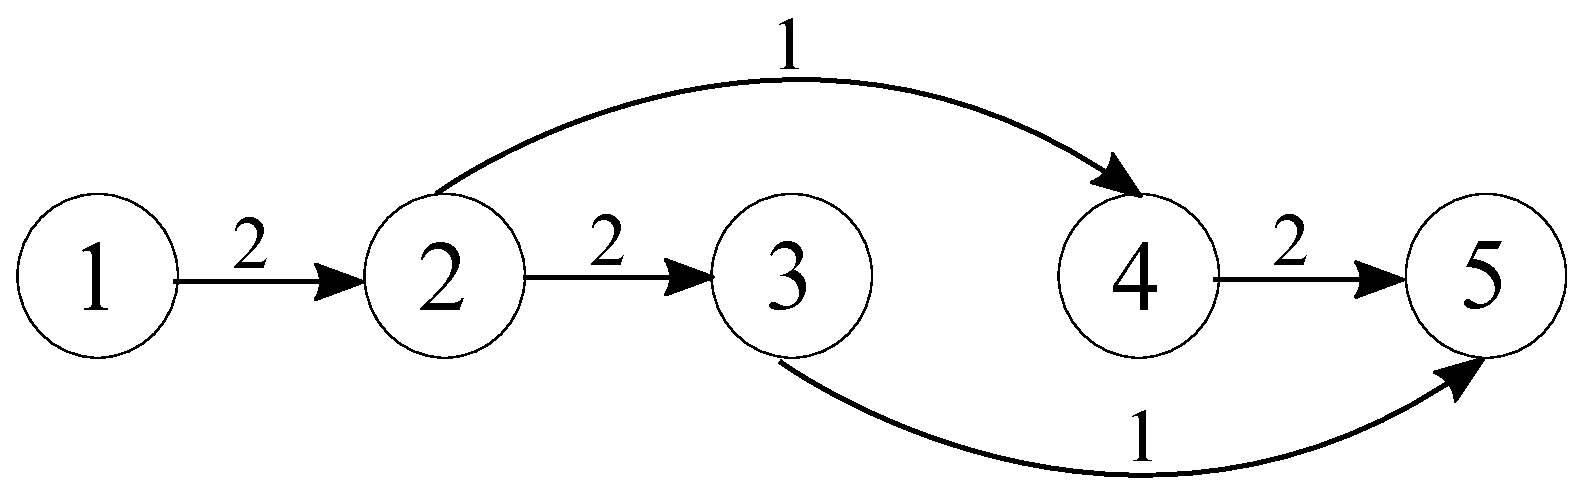
\includegraphics[width=0.9\textwidth]{example1}
	\end{center}
	\caption{Граф $G$.}
	\label{fig:picg}
\end{figure}
\par Для этого графа $X = \{1, 2, 3, 4, 5\}$, $C = \{1, 2\}$. Этот граф не имеет кратных дуг, поэтому их можно представлять как пары $(x, y)$ вершин графа, где $x$ -- начало дуги, $y$ -- её конец. Каждая дуга допускает ровно один цвет, надписанный над ней. Таким образом, $U =\{(1, 2), (2, 3), (2, 4), (3, 5), (4, 5)\}$, $U_1 =\{(2, 4), (3, 5)\}$, $U_2 =\{(1, 2), (2, 3), (4, 5)\}$. Непосредственно можно убедиться, что граф $G$ не содержит контуров, а его вершины топологически упорядочены.
\par Пусть $s = 1$, $t = 5$, а стохастическая матрица $P$ имеет вид:
\[P = \begin{pmatrix} 
0,7 & 0,3\\ 
0,3 & 0,7 
\end{pmatrix}
\]
\par Применяя вышеизложенный алгоритм, найдём матрицу вероятностей $P^{(1)}$ для вершины $s = 1$, а также стратегию $(v_{i, n})_{1 \le n < 5, i = 1, 2}$.
\par Для вершины $5$ имеем:
\[P^{(5)} = E = \begin{pmatrix} 
1 & 0\\ 
0 & 1 
\end{pmatrix}
\]
\par Для дальнейшего нам понадобится одно обозначение.
\par Будем обозначать $L_k(A)$ взятие $k$-й строки матрицы $A$, т.е. 
\[L_k((a_{i,j})_{i,j = 1}^{M}) = (a_{k, 1}, a_{k, 2}, ..., a_{k, M}).\]
\par Из определения умножения матриц следует, что:
\[
L_k(A \cdot B) = L_k(A) \cdot B.
\]
\par Для вершины $4$ имеем $X_1(4) = \emptyset$, поэтому $v_{1, 4} = \bigotimes$.
\par $X_2(4) = \{5\}$, поэтому: 
\[L_2(P^{(4, 5)}) = L_2(P) \cdot P^{(5)} = \begin{pmatrix} 0,3 & 0,7 \end{pmatrix} \begin{pmatrix} 1 & 0\\ 0 & 1 \end{pmatrix} = \begin{pmatrix} 0,3 & 0,7 \end{pmatrix} \]
\par Здесь $v_{2, 4} = 5$ как единственная вершина множества $X_2(4)$.
\par Таким образом, 
\[
P^{(4)} = \begin{pmatrix} 0 & 0\\ 0,3 & 0,7 \end{pmatrix}.
\]

\par Для вершины $3$ имеем $X_1(3) = \{5\}$, поэтому: 
\[L_1(P^{(3, 5)}) = L_1(P) \cdot P^{(5)} = \begin{pmatrix} 0,7 & 0,3 \end{pmatrix} \begin{pmatrix} 1 & 0\\ 0 & 1 \end{pmatrix} = \begin{pmatrix} 0,7 & 0,3 \end{pmatrix} \]
\par Здесь $v_{1, 3} = 5$ как единственная вершина множества $X_1(3)$.
\par $X_2(3) = \emptyset$, поэтому $v_{2, 3} = \bigotimes$.
\par Таким образом, 
\[
P^{(3)} = \begin{pmatrix} 0,7 & 0,3\\ 0 & 0 \end{pmatrix}.
\]

\par Для вершины $2$ имеем $X_1(2) = \{4\}$, поэтому: 
\[L_1(P^{(2, 4)}) = L_1(P) \cdot P^{(4)} = \begin{pmatrix} 0,7 & 0,3 \end{pmatrix} \begin{pmatrix} 0 & 0\\ 0,3 & 0,7 \end{pmatrix} = \begin{pmatrix} 0,09 & 0,21 \end{pmatrix} \]
\par Здесь $v_{1, 2} = 4$ как единственная вершина множества $X_1(2)$.
\par $X_2(2) = \{3\}$, поэтому: 
\[L_2(P^{(2, 3)}) = L_2(P) \cdot P^{(3)} = \begin{pmatrix} 0,3 & 0,7 \end{pmatrix} \begin{pmatrix} 0,7 & 0,3\\ 0 & 0 \end{pmatrix} = \begin{pmatrix} 0,21 & 0,09 \end{pmatrix} \]
\par Здесь $v_{2, 2} = 3$ как единственная вершина множества $X_2(2)$.
\par Таким образом, 
\[
P^{(2)} = \begin{pmatrix} 0,09 & 0,21\\ 0,21 & 0,09 \end{pmatrix}.
\]

\par Для вершины $1$ имеем $X_1(1) = \emptyset$, поэтому $v_{1, 1} = \bigotimes$.
\par $X_2(1) = \{2\}$, поэтому: 
\[L_2(P^{(1, 2)}) = L_2(P) \cdot P^{(2)} = \begin{pmatrix} 0,3 & 0,7 \end{pmatrix} \begin{pmatrix} 0,09 & 0,21\\ 0,21 & 0,09 \end{pmatrix} = \begin{pmatrix} 0,174 & 0,126 \end{pmatrix} \]
\par Здесь $v_{2, 1} = 2$ как единственная вершина множества $X_2(1)$.
\par Таким образом, 
\[
P^{(1)} = \begin{pmatrix} 0 & 0\\ 0,174 & 0,126 \end{pmatrix}.
\]
\par Как мы видим, в случае, если путешественник находится в стартовой вершине в цвете $1$, он не сможет достичь вершины $5$ ни при каком условии: $p_1 = 0$. Если же он изначально находится в цвете $2$, он может достичь вершины $5$ с вероятностью $p_2 = 0,174 + 0,126 = 0,3$. Найденные вершины стратегии укажут путешественнику наиболее оптимальный маршрут.
	
	\newpage
	
  %% стилевой файл для оформления по ГОСТу
%\bibliography{biblio}     %% имя библиографической базы (bib-файла) 

\begin{thebibliography}{}
	\bibitem{berzh}  Берж, К. Теория графов и ее применения. / Берж К.-- М.: Издательство иностранной литературы, 1962.-- 320 с.
	\bibitem{sinkit}  Галина Мурсалиева. Группы смерти (18+) / Галина Мурсалиева // Новая газета.-- URL: https://www.novayagazeta.ru/articles/2016/05/16/68604-gruppy-smerti-18.-- 2016.
	\bibitem{stargraph}  Емцева, Е.Д., Солодухин, К.С. Дискретная математика. Часть 3 (Курс лекций). / Емцева, Е.Д., Солодухин, К.С. // URL: https://abc.vvsu.ru/books/l\_diskrmat3/page0008.asp
	\bibitem{erus}  Ерусалимский, Я.М. Дискретная математика. Теория, задачи, приложения: учеб. пособие / Я.М. Ерусалимский.-- М.: Вузовская книга, 2009.-- 288 с.
	\bibitem{harari} Лекции по теории графов. / Емеличев В. А. [и др.] -- М.: Наука, 1990. -- 384 с.	
	\bibitem{izom}  Laszlo Babai. Graph Isomorphism in Quasipolynomial Time / Laszlo Babai // 2015.
	\bibitem{gitbook} Loeliger, J., McCullough, M. Version Control with Git. / Jon Loeliger, Matthew McCullough.-- Sebastopol: O'Reilly, 2012.-- 436p.
	\bibitem{pythdoc} Python 3.6.5 documentation. // URL: https://docs.python.org/3/index.html.
	\bibitem{bellmanford} R. Bellman: On a Routing Problem // Quarterly of Applied Mathematics. 1958. Vol 16, No. 1. C. 87-90, 1958.
	\bibitem{patmat}  Towards Practical and Robust Labeled Pattern Matching in Trillion-Edge Graphs / Tahsin Reza [и др.] // 2017.
	\bibitem{graphtool} Welcome to graph-tool’s documentation! // URL: https://graph-tool.skewed.de/static/doc/index.html.
\end{thebibliography}

\end{document}